\documentclass[]{article}
\usepackage{lmodern}
\usepackage{amssymb,amsmath}
\usepackage{ifxetex,ifluatex}
\usepackage{fixltx2e} % provides \textsubscript
\ifnum 0\ifxetex 1\fi\ifluatex 1\fi=0 % if pdftex
  \usepackage[T1]{fontenc}
  \usepackage[utf8]{inputenc}
\else % if luatex or xelatex
  \ifxetex
    \usepackage{mathspec}
  \else
    \usepackage{fontspec}
  \fi
  \defaultfontfeatures{Ligatures=TeX,Scale=MatchLowercase}
\fi
% use upquote if available, for straight quotes in verbatim environments
\IfFileExists{upquote.sty}{\usepackage{upquote}}{}
% use microtype if available
\IfFileExists{microtype.sty}{%
\usepackage[]{microtype}
\UseMicrotypeSet[protrusion]{basicmath} % disable protrusion for tt fonts
}{}
\PassOptionsToPackage{hyphens}{url} % url is loaded by hyperref
\usepackage[unicode=true]{hyperref}
\hypersetup{
            pdftitle={Integrating terminal element variability into WBE},
            pdfborder={0 0 0},
            breaklinks=true}
\urlstyle{same}  % don't use monospace font for urls
\usepackage[margin=1in]{geometry}
\usepackage{graphicx,grffile}
\makeatletter
\def\maxwidth{\ifdim\Gin@nat@width>\linewidth\linewidth\else\Gin@nat@width\fi}
\def\maxheight{\ifdim\Gin@nat@height>\textheight\textheight\else\Gin@nat@height\fi}
\makeatother
% Scale images if necessary, so that they will not overflow the page
% margins by default, and it is still possible to overwrite the defaults
% using explicit options in \includegraphics[width, height, ...]{}
\setkeys{Gin}{width=\maxwidth,height=\maxheight,keepaspectratio}
\IfFileExists{parskip.sty}{%
\usepackage{parskip}
}{% else
\setlength{\parindent}{0pt}
\setlength{\parskip}{6pt plus 2pt minus 1pt}
}
\setlength{\emergencystretch}{3em}  % prevent overfull lines
\providecommand{\tightlist}{%
  \setlength{\itemsep}{0pt}\setlength{\parskip}{0pt}}
\setcounter{secnumdepth}{0}
% Redefines (sub)paragraphs to behave more like sections
\ifx\paragraph\undefined\else
\let\oldparagraph\paragraph
\renewcommand{\paragraph}[1]{\oldparagraph{#1}\mbox{}}
\fi
\ifx\subparagraph\undefined\else
\let\oldsubparagraph\subparagraph
\renewcommand{\subparagraph}[1]{\oldsubparagraph{#1}\mbox{}}
\fi

% set default figure placement to htbp
\makeatletter
\def\fps@figure{htbp}
\makeatother


\title{Integrating terminal element variability into WBE}
\author{}
\date{\vspace{-2.5em}}

\begin{document}
\maketitle

The assumption of invariance of terminal tips effectively leads to the
assumption that the number of terminal elements is proportional to the
metabolic capacity of the network, or \(n_{N} \propto V_{N}^{L}\).
Estimates of metabolic scaling fail because this is not the case, as
we've shown previously. Returning to the original scaling argument, the
result of applying a geometric series to the network model is

\begin{equation}
\label{eq:1}
V_{N}C_{0}N_{N}^{4/3} = V_{net}
\end{equation}

One approach to allowing variation in terminal tips is to replace
\(V_{N}\) with a series of random variables
\(\overline{r_{k}}^{2} \overline{l_{k}} \pi = \overline{V_{N}}\), where
\(\overline{V_{N}}\) now represents the average terminal tip volume for
a vascular network. Substituting directly into the expression resulting
from the geometric series we have

\[\overline{V_{N}}N_{N}^{4/3} = V_{net}\]
\[N_{N}^{4/3} = V_{net}/\overline{V_{N}}\]

\begin{equation}
\label{eq:2}
N_{N} \propto (V_{net}/\overline{V_{N}})^{3/4}
\end{equation}

where \(\overline{V_{N}}\) is included in the scaling relationship
because the average volume of terminal tips may very within and across
vascular networks. We computed this correction to the empirical scaling
by quantifying \(\overline{V_{N}}\) as the geometric mean in volumes of
distal terminal tips for a given (sub)tree. However, this approach
fails. This is likely because variability in terminal tips propagates
and scales throughout the network, proper accounting of which
necessitates revising the geometric series.

Here, we attempt to modify the derivation using the geometric series,
incorporating new scaling ratios intended to account for variability in
terminal tip dimensions across a network.

First, we return to the definition of space filling in the context of
length scaling:

\begin{equation}
\frac{N_{k}l_{k}^{3}}{N_{k+1}l_{k+1}^{3}} = 1 
\end{equation}

This statement formalizes the concept of a `service volume' in WBE, and
provides the definition for the length scaling ratio
\(\gamma = \frac{l_{k+1}}{l_{k}}\) in terms of the branching ratio
\(n = \frac{N_{k+1}}{N_{k}}\):

\[\frac{N_{k+1}l_{k+1}^{3}}{N_{k}l_{k}^{3}} = 1\] \[n\gamma^{3} = 1\]
\[\gamma = n^{-1/3}\]

Our intuition is that modifying the definition of \(\gamma\) will allow
tip variability to enter into the theory, and particularly to propagate
iteself through the geometric series. Now we introduce a length
deviation factor for any branch at depth k as

\begin{equation}
\gamma^{*} = \frac{l_k}{\overline{l_{k}}}
\end{equation}

which is the ratio of the branch length to the mean length
\(\overline{l_{k}}\) at depth k.

How is this related to terminal tip variability? If the expression for
\(\gamma^{*}\) is true, then

\[l_{k} = \overline{l_{N}}(\gamma^{*})^{N-k}\]

will also be true. This allows us to link tip variability (in the form
of random variables \(\overline{l_{N}}\) and more generally
\(\overline{l_{k}}\)) to any level of the network using the scaling
ratio \(\gamma^{*}\). However we have no proof of this and it is
questionable, since unlike \(\gamma\), \(\gamma^{*}\) must vary
throughout the network. This makes it more difficult to link the
terminal level of the hierarchy N with an arbitrary level k, which is
the power of symmetry and the geometric series in WBE. Therefore, some
other definition of \(\gamma^{*}\) may be more appropriate.

However, if terminal element variability has an effect on scaling then
some factor like \(\gamma^{*}\) must exist. The intention is to
introduce a new scaling ratio that might modify our predictions for
metabolic scaling by integrating it into the geometric series. In order
to do this, we need to express the new scaling ratio in terms of the
branching ratio n. In the symmetric case (equivalent terminal tips) we
would expect \(\gamma^{*} = 1\), where for each branch level l,
\(l_{k} = \overline{l_{k}}\). Then, if \(\gamma^{*} = n^{-x}\), then in
the symmetric case \(x = 0\) so that \(\gamma^{*} = 1\) has no overall
effect on the scaling of the network and `drops out' of the theory.
Thus, our first major prediction is that \(x \neq 0\), and we propose to
test this using the relationship

\[x = \frac{log \gamma^{*}}{log n}\]

Furthermore, if the definition for \(\gamma^{*}\) holds true, we can
show that the characteristic exponent \(x\) shows up in the final
expression for metabolic scaling of the number of terminal tips
\(n_{N}\) such that

\[n_{N} \propto V_{net}^{3/4 + x}\]

Likewise, an independent scale factor for terminal radii could be
incorporated, but there is some evidence that variation in terminal
elements is primarily driven by variation in lengths in LiDAR scans of
trees. Furthermore, the concept of service volumes is inherently related
to length scaling so we limit our investigation to the new factor
\(\gamma^{*}\) for the time being.

If our two predictions for the value \(x\) are well-supported, it may be
worthwhile to incorporate the new scale factor into expressions for
\(\theta\) including other branching traits. Currently, the assumptions
involved in the definition for \(\gamma^{*}\) are not clear, and the
nature of the definition may need to change to more properly account for
variation in terminal element geometry at each level of the network.

A major problem is that \(\gamma^{*}\) is not a compensatory factor. Any
variation in terminal tips will result in a reduction of the metabolic
scaling exponent below 3/4. This would be consistent with our results
from tip counting, but volume scaling regressions indicate that we
should still expect a 3/4 scaling result. All that \(\gamma^{*}\) can do
is allow us to once again make predictions using the original, symmetric
WBE theory based on integer counts of terminal elements. However, if
using \(\gamma^{*}\) allows us to recover the original theory, we have
evidence that terminal tip variability may be heavily contributing to
observed variation in metabolic scaling exponents. Below, we attempt to
quanity \(\gamma^{*}\) and evaluate the predictions it entails.

First, the variation in \(\gamma^{*}\) is consistent with a long tail in
the geometry of branches, such that a few large branches pollute data on
many small terminal elements

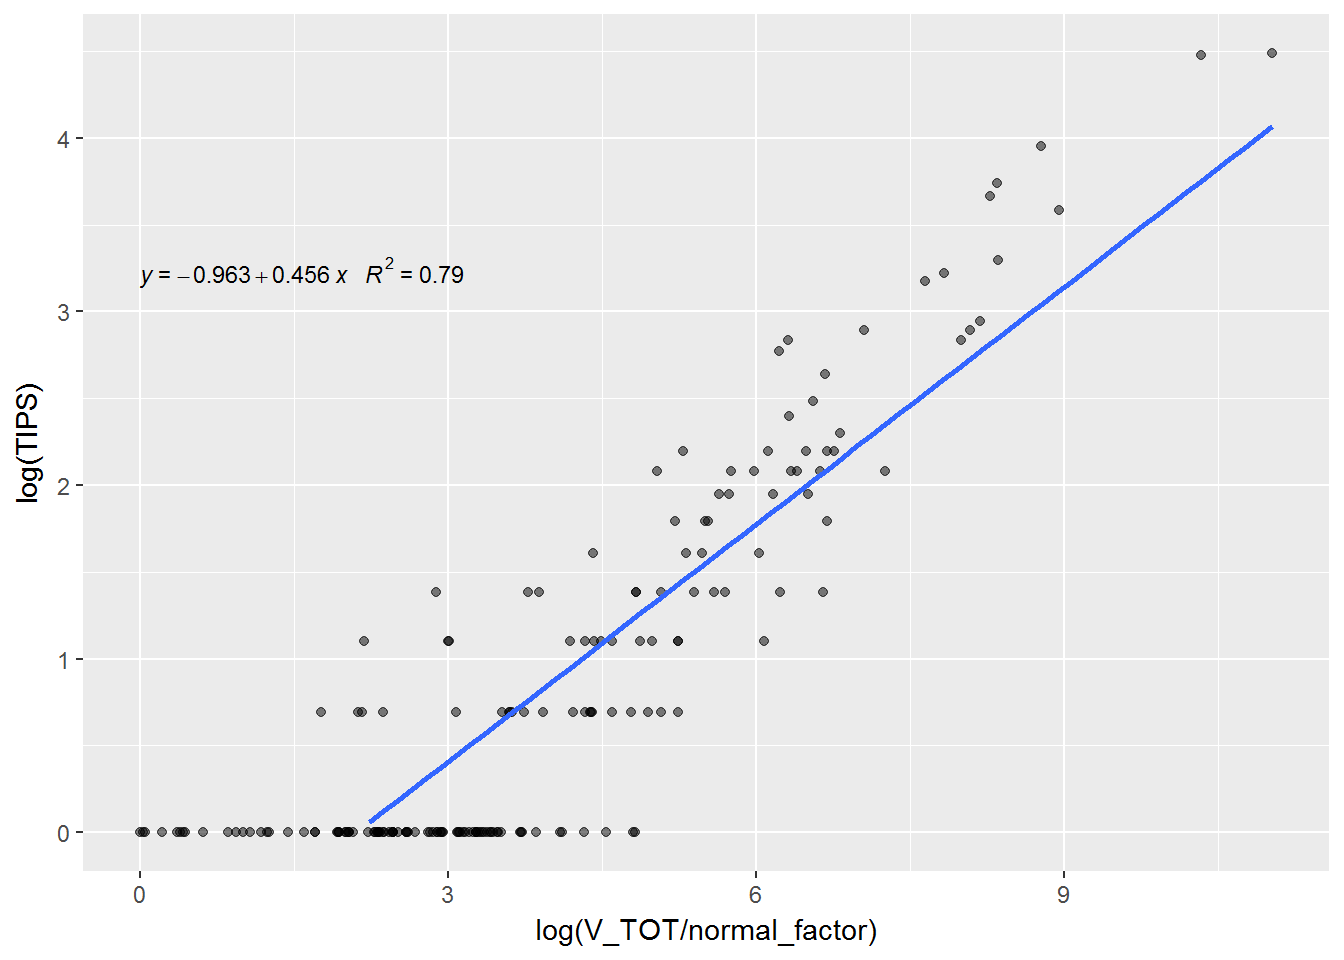
\includegraphics[width=800px]{tip_scaling_pt2_files/figure-latex/unnamed-chunk-1-1}

To evaluate this theory, our goal is to improve on the relationship
between tip scaling exponents and volume scaling exponents shown here

\includegraphics[width=800px]{tip_scaling_pt2_files/figure-latex/unnamed-chunk-2-1}
We would predict a slope of 1 between these two axes, but the slope is
shallow and the trend line exhibits significant scatter.

We calculated a mean value of \(x\) for each tree by computing
\[\frac{log \gamma^{*}}{log n}\] at each node, and taking the mean value
of this exponent across all nodes. Then, we applied the \(x\) value as a
correction to the `true' metabolic scaling exponent calculated from
volume scaling regressions. Below, we regress this corrected scaling
exponent against tip scaling exponents (based on the integer number of
distal tips across subtrees)

\includegraphics[width=800px]{tip_scaling_pt2_files/figure-latex/unnamed-chunk-3-1}

The addition of the scaling ratio \(\gamma^{*}\) is moderately
successful, to the extent that it steepens the slope between tip
counting scaling exponents and corrected volume scaling exponents (from
a slope of \textasciitilde{}0.47 to a slope of about
\textasciitilde{}0.71). However, the method seems to add more
variability to the dataset and increases the scattter, reducing the
adjusted \(R^{2}\) fit quality.

\end{document}
